\subsection{ماشین مجازی}
در ابتدا به کمک دستور زیر تست می‌کنیم که آیا از سمت
\lr{host}
می‌توان به دیتابیس
\lr{guest}
وصل شد یا خیر. در صورتی که این دستور با خطا مواجه شود، باید تنظیمات دسترسی از
\lr{host}های
مختلف را مانند مقدمه بررسی کرد. به عنوان مثال در شکل
\ref{fig:postgres:vm:connection}
من از
\lr{host} به \lr{guest}
وصل شدم.
\begin{figure}[H]
    \centering
    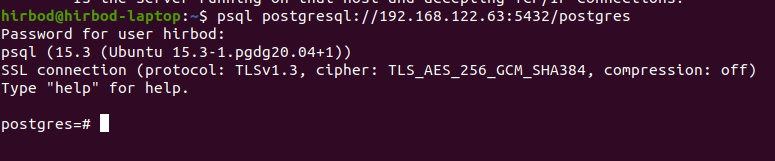
\includegraphics[scale=0.5]{pictures/postgres/vm/connection.png}
    \caption{وصل شدن از host به guest در PostgreSQL}
    \label{fig:postgres:vm:connection}
\end{figure}
برای ماشین مجازی نیز مانند ماشین حقیقی تنظیمات مشابهی با شکل
\ref{fig:postgres:vm:connection:hammerdb}
انجام می‌دهیم.
\begin{figure}[H]
    \centering
    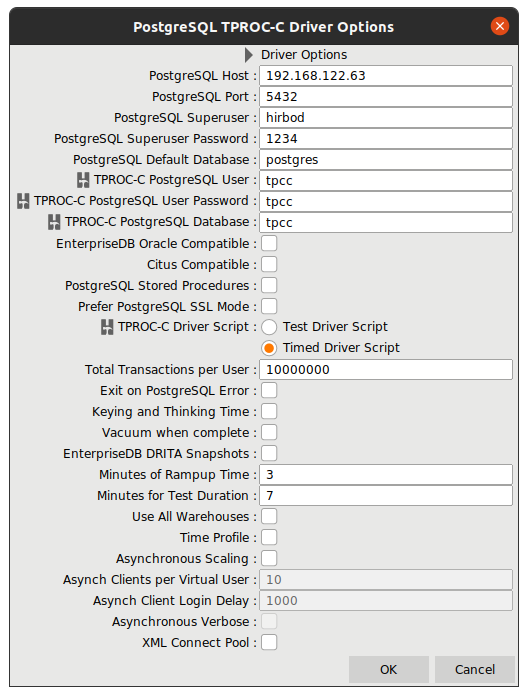
\includegraphics[scale=0.42]{pictures/postgres/vm/connection-hammerdb.png}
    \caption{تنظیمات وصل شدن در HammerDB}
    \label{fig:postgres:vm:connection:hammerdb}
\end{figure}
سپس صرفا برای هر کرنل تست را انجام می‌دهیم.